% 3DCGR Latex Template for Assignment Docs
% Florian Michelic and Reinhold Preiner, October 2021
%-------------------------------------------------------------------

\documentclass{article}
\usepackage[utf8]{inputenc}
\usepackage{hyperref}
\usepackage{cite}
\usepackage[english]{babel}
 \usepackage{hyperref}
\usepackage[nottoc]{tocbibind}
\usepackage{subfig}
\usepackage{graphicx}
\usepackage{placeins}
\usepackage{hyperref}


\usepackage{geometry}
\geometry{margin=1in}

\hypersetup{
    colorlinks=true,
    linkcolor=blue,
    filecolor=magenta,      
    urlcolor=cyan,
    citecolor = black,
}

\usepackage{comment}

\title{	
	\large Simulation \& Animation - SS 2022\\
	\Huge{Magic Eight}\\
	\huge{Game Concept}
}
\author{\parbox{\textwidth}{\centering
	Dominik V\"olkel, 11811035, d.voelkel@student.tugraz.at\\%
	Phillip Stranger, 11807773, phillip.stranger@student.tugraz.at\\%
}}
\date{\today}


\begin{document}

\maketitle

\section{Game Concept}

Basically super mario power ups meet 8-ball pool.\\
The basic idea is that two players play 8-ball pool against each other with somewhat normal rules and the twist is that at some point in the game, either via pickup or some other mechanic, chaos is increased on the pool table with some power ups that change some underlying property of the game. \\

In general everything is controlled with the mouse via drag/drop motions.

Examples of somewhat normal properties that may be changed:

\begin{itemize}
	\item Table Friction $\rightarrow$ Change the friction of individual balls on the table.
	\item Mass $\rightarrow$ Change the mass and gravity of individual balls or positions of the table and their gravitational pull on other objects.
	\item Shape $\rightarrow$ Objects still perform like pool balls but have a rectangular or other-wisely shaped hitbox making otherwise impossible shots/collisions possible.
	\item Changing Wall 'bouncyness' $\rightarrow$ Change how hard an object bounces from another object or the boarder wall of the game space.
	\item Size $\rightarrow$ Change the size of an object or the size of the 'hole' or the size of the entire playing field.
	\item High power/collision power $\rightarrow$ change the rules of normal collision such that small impacts have huge effects.
	\item Introduce other objects  $\rightarrow$ Introduce stationary (immovable) or breakable objects to the scene.
\end{itemize}



More fun and weird effects with quirky power ups:
\begin{itemize}
\item 'bind' two balls together  $\rightarrow$ bind two objects/balls together with a bouncy/elastic string/cord making them have an effect on one another
\item different 'shooting' mechanisms  $\rightarrow$ instead of using a pool cue to fire the ball rather the ball fires a suction cup onto another ball which makes the hit ball speed towards the first.
\item "Super mario star" $\rightarrow$ Any ball touched by this effect is instantly deleted and respawns at some dedicated position.
\item Game balance $\rightarrow$ Increase/decrease your/your opponents ball count or change designated final holes.
\item "Wrong game" $\rightarrow$ roll a bowling ball down the middle of the playing field pushing all other objects out of the way.
\item "Higher power" $\rightarrow$ place very strong gravitational objects (like a black hole) somewhere on the playing field or influence the field permanently in another way.
\item "follow me" $\rightarrow$ designating two objects which are now in hierarchical relation to another. E.g. if A is made the parent of B the n B moves if A moves but B does not influence A (unless directly hit). This is a point for point description of implementing on the fly hierarchical transformations.
\end{itemize}

Of course none of these power ups should make the game impossible to win for any party, but they might make it very difficult and unfair.

The following figures are sketches trying to visualize some effects.

\begin{figure*}[!htb]
\centering
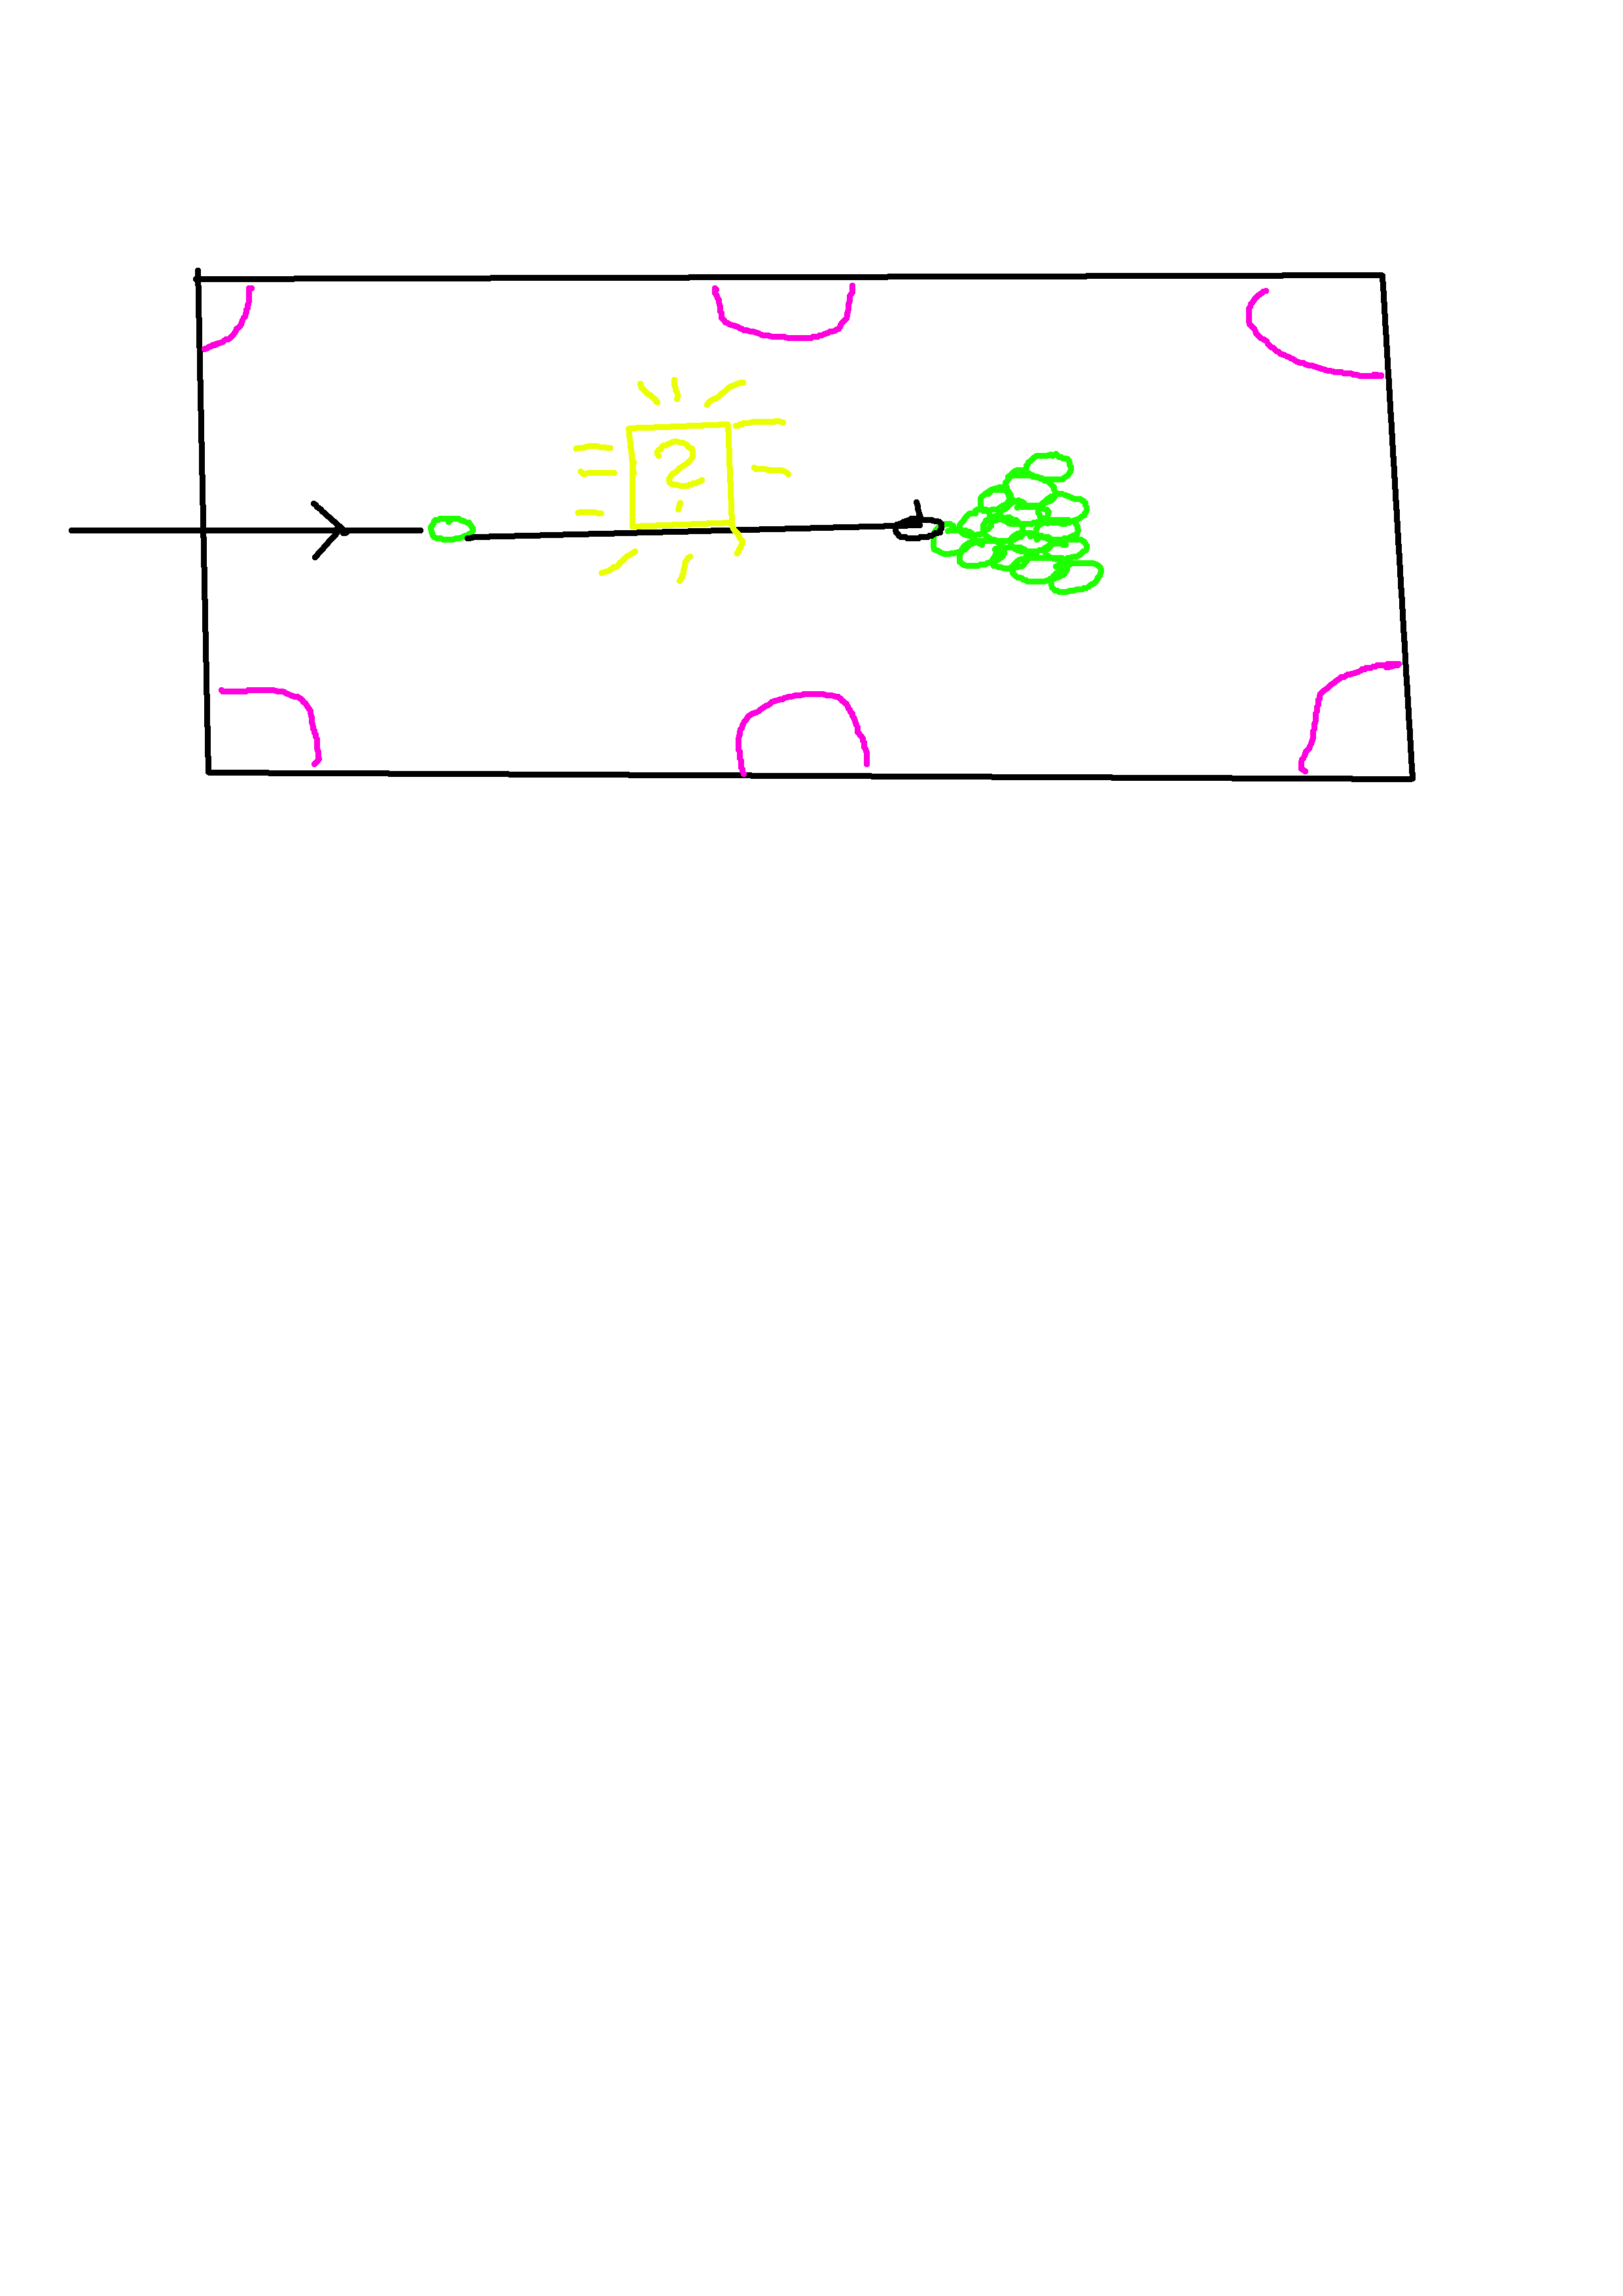
\includegraphics[trim={2cm 17cm 2cm 2cm},width=0.6\textwidth,clip]{img/game_state_0.png}
\caption{Basic game start state sketch. Normal pool but with a yellow "power up" box in the path of the white ball. The black arrow symbolizes a pool cue and the predicted trajectory in black.}
\label{fig:game_state_0}
\end{figure*}

\begin{figure*}[!htb]
	\centering
	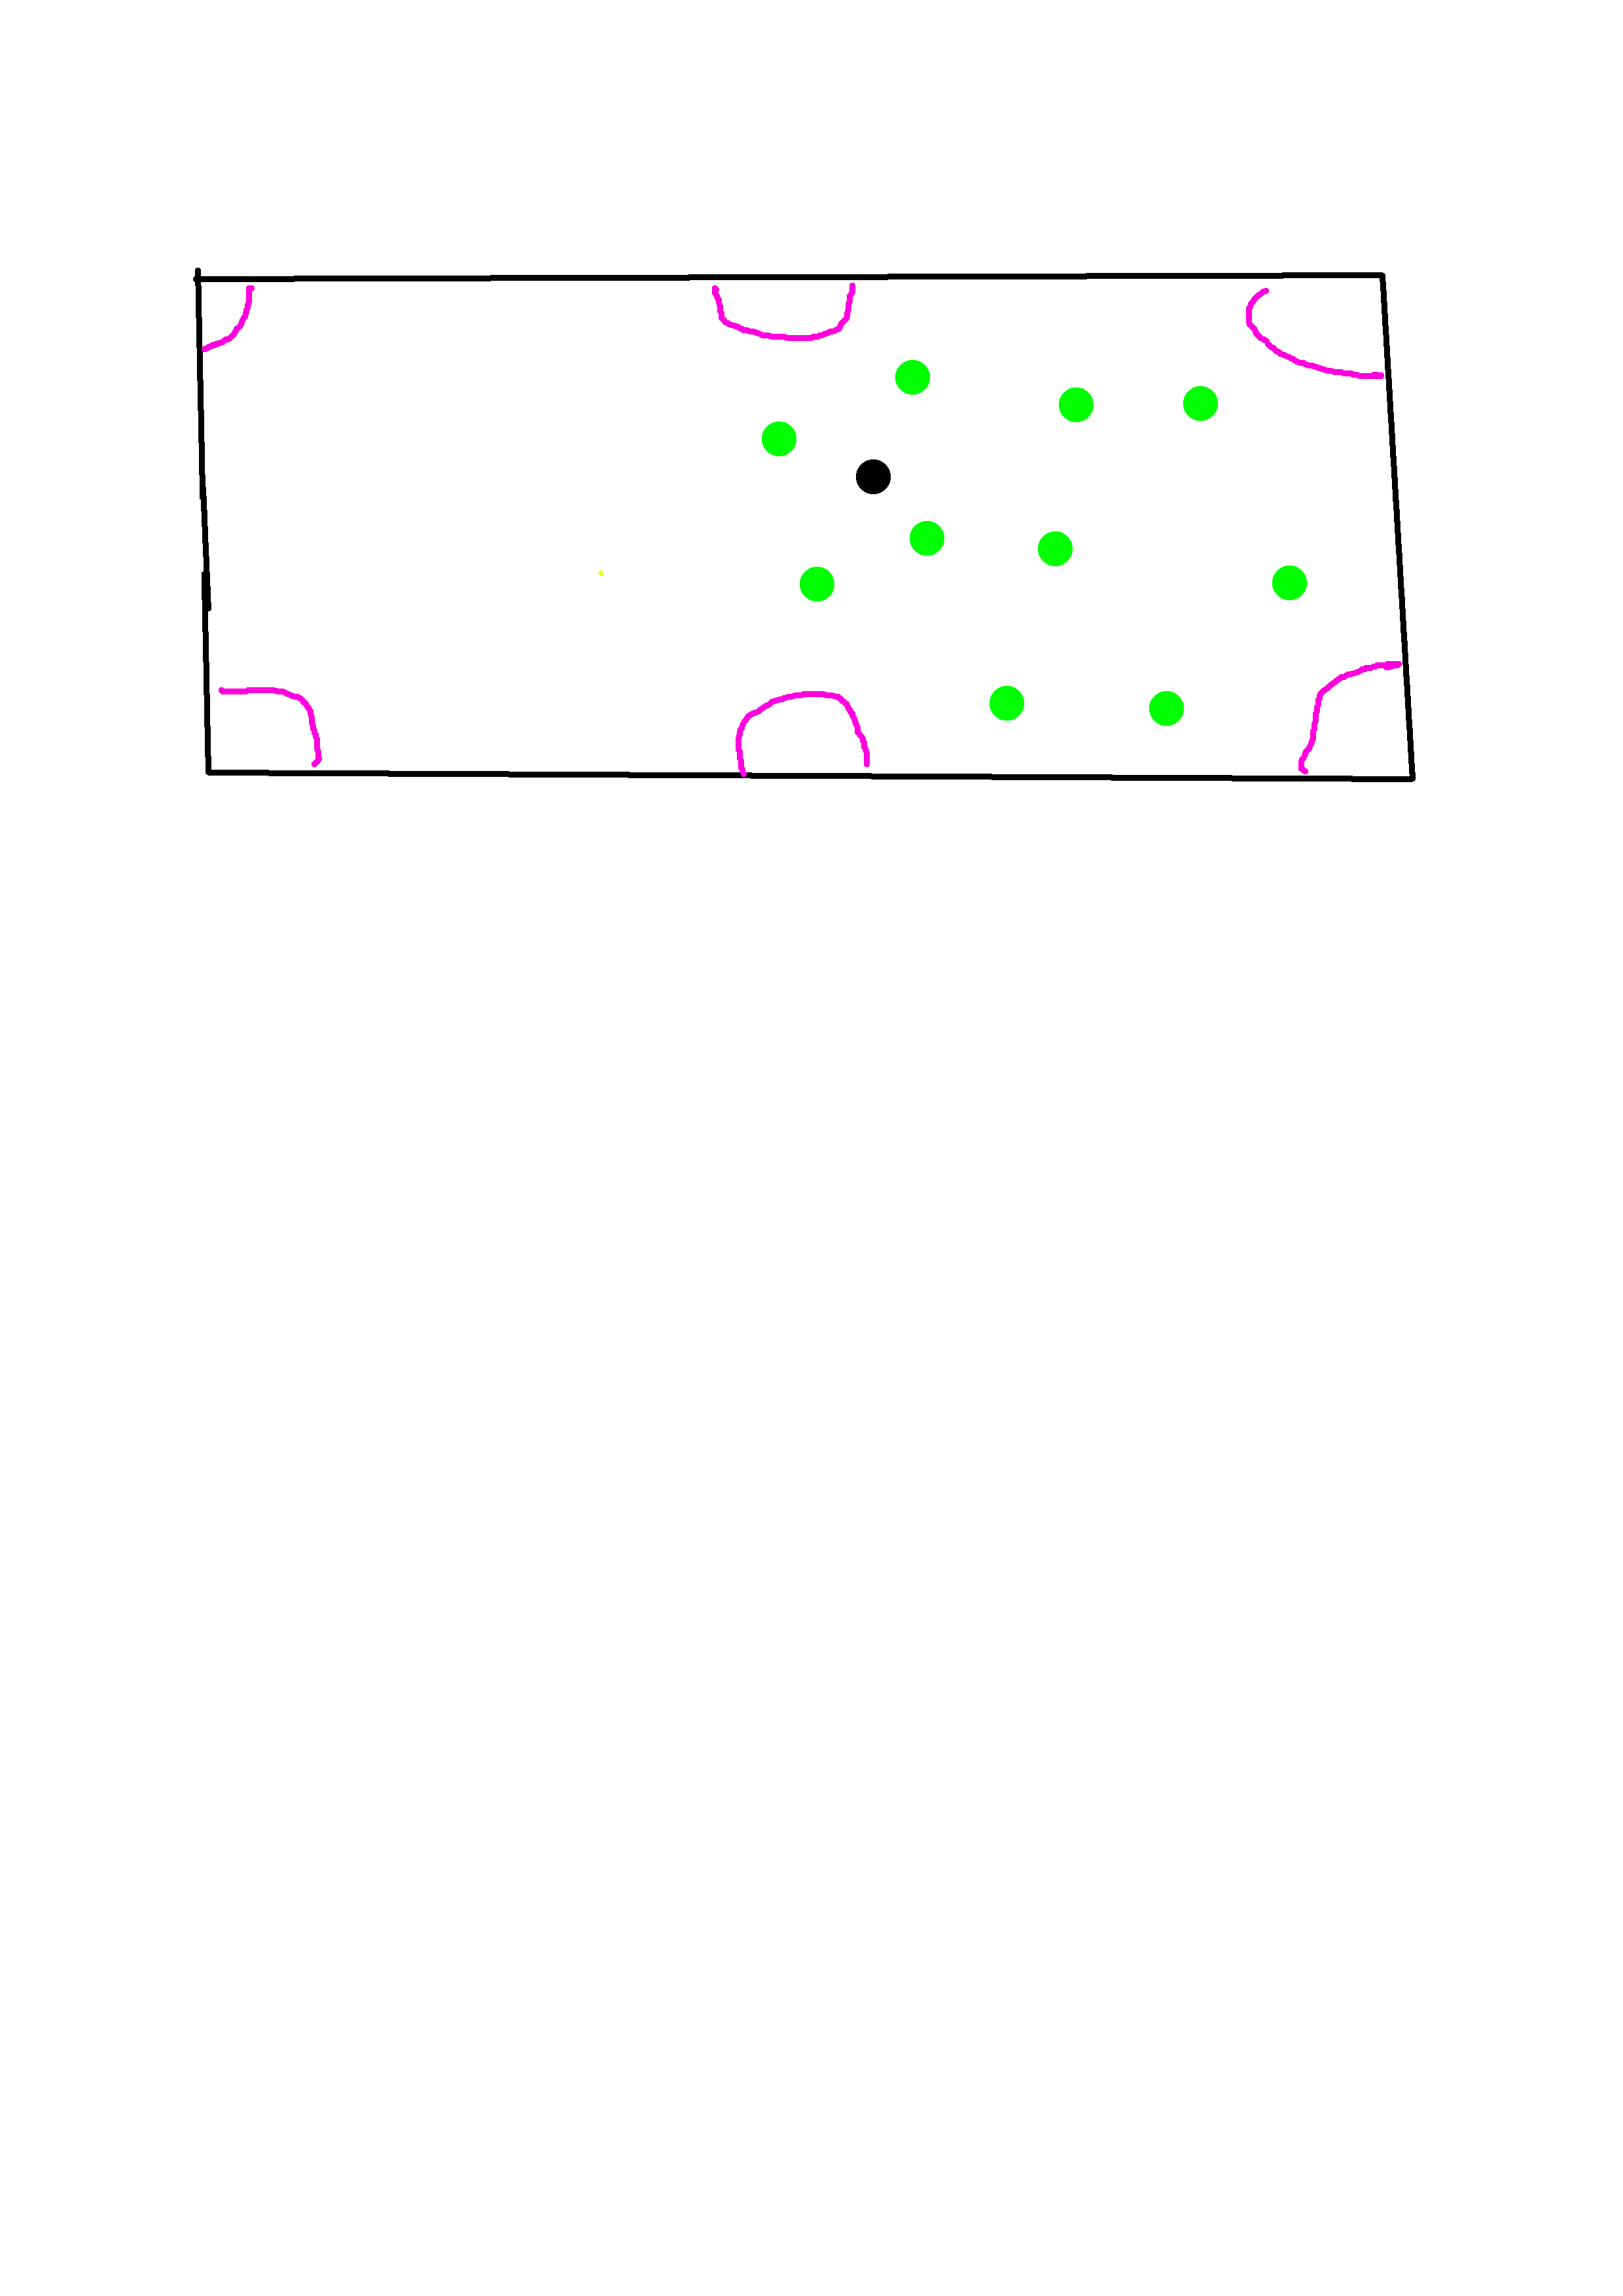
\includegraphics[trim={2cm 17cm 2cm 2cm},width=0.6\textwidth,clip]{img/game_state_1.png}
	\caption{Representation of some random game state, the exact ball numbers etc. does not matter.}
	\label{fig:game_state_1}
\end{figure*}

\begin{figure*}[!htb]
	\centering
	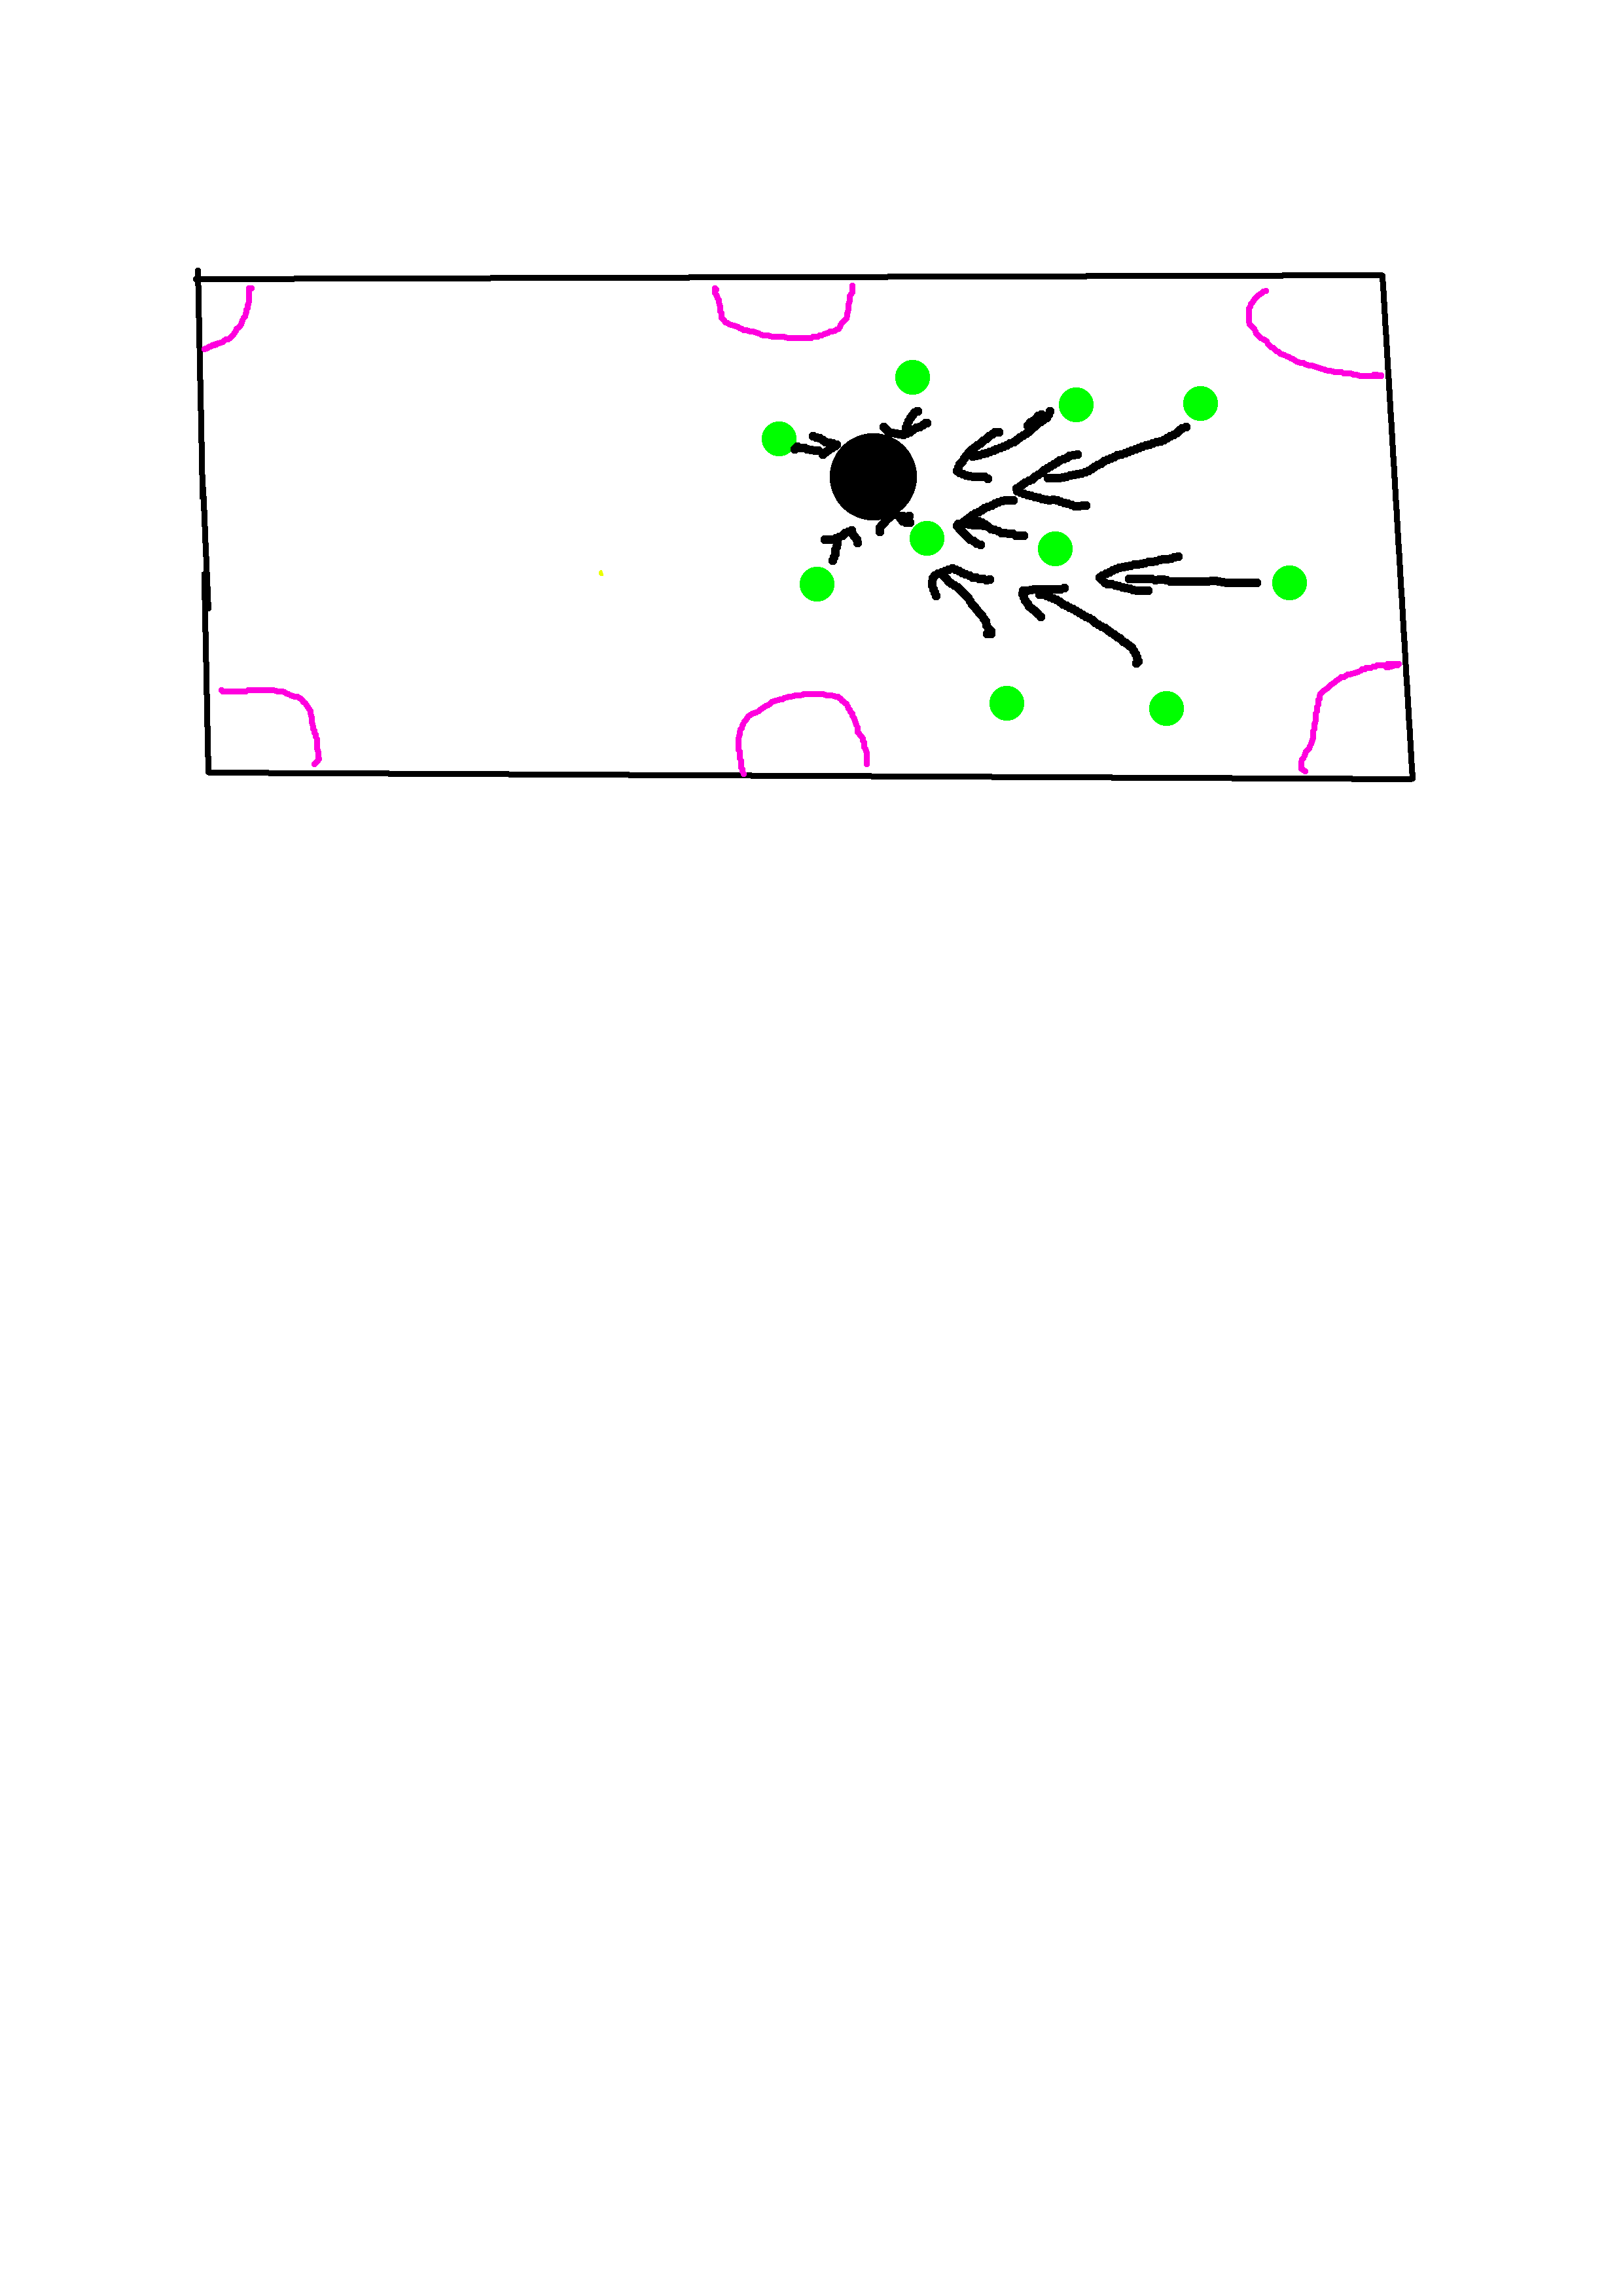
\includegraphics[trim={2cm 17cm 2cm 2cm},width=0.6\textwidth,clip]{img/game_state_2.png}
	\caption{The ball marked in black had its mass increased for a limited time attracting all other balls on the field.}
	\label{fig:game_state_2}
\end{figure*}

\begin{figure*}[!htb]
	\centering
	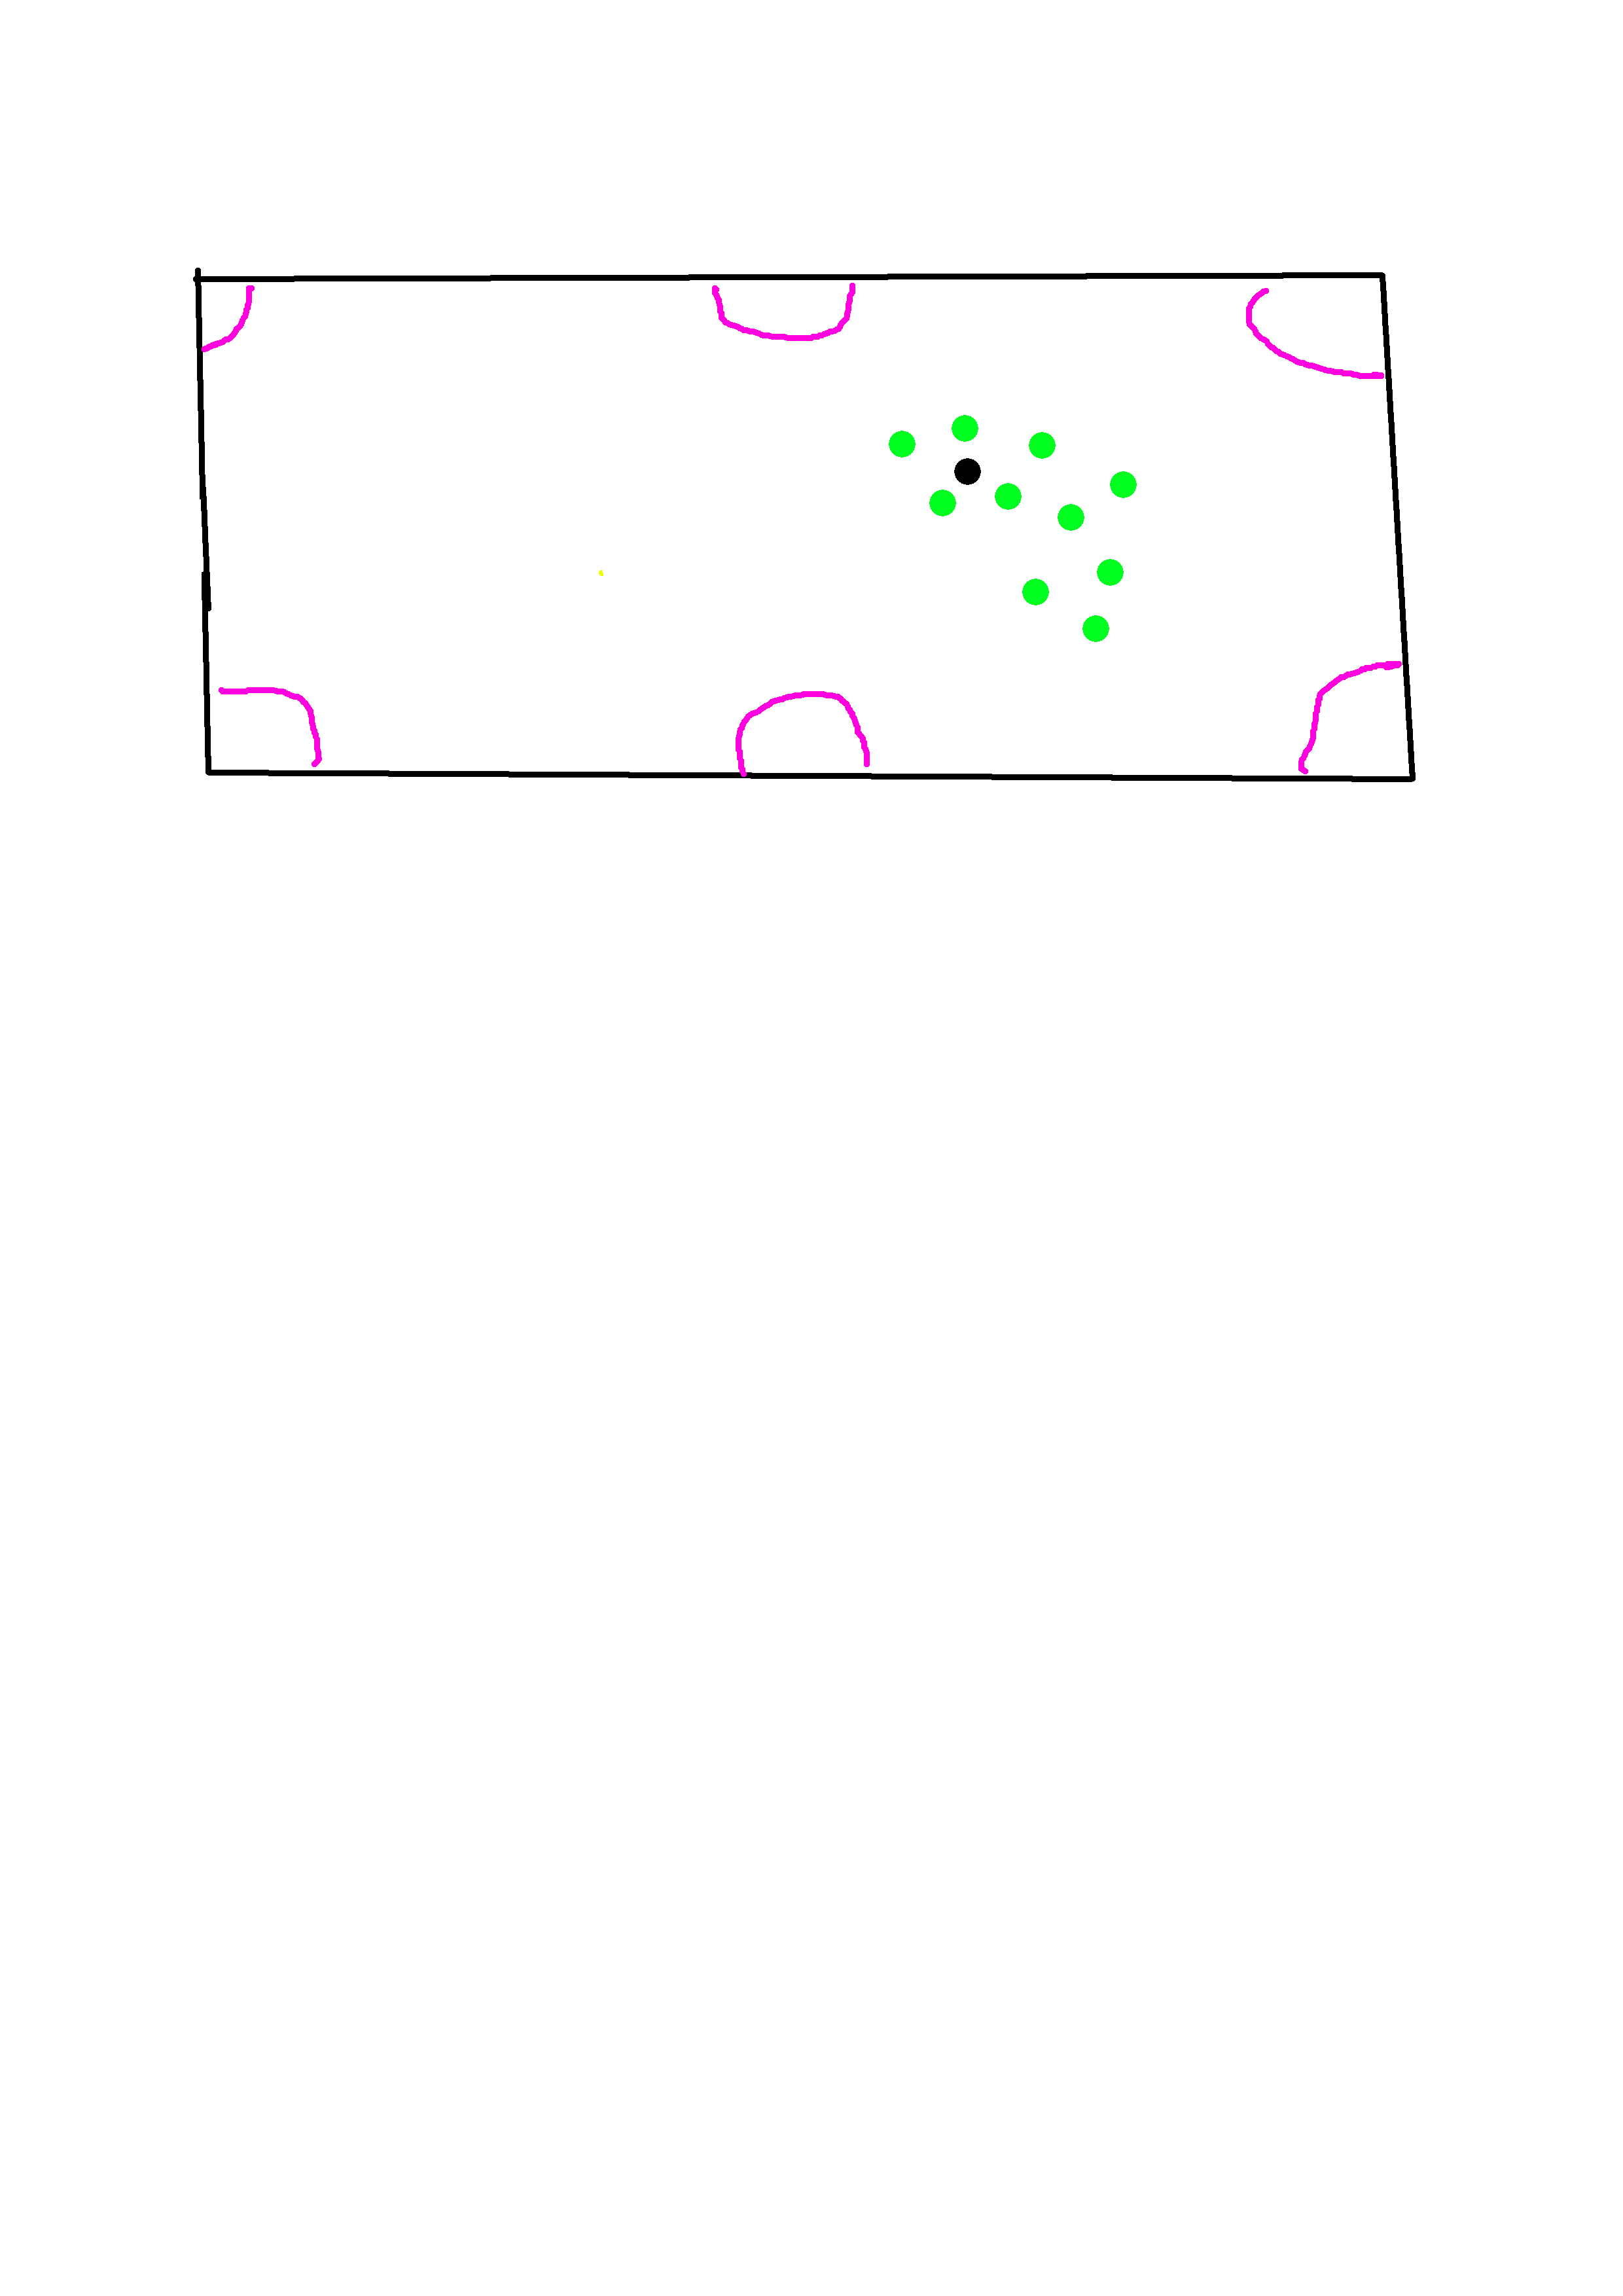
\includegraphics[trim={2cm 17cm 2cm 2cm},width=0.6\textwidth,clip]{img/game_state_3.png}
	\caption{After the attraction effect has ended the balls have settled into their new location.}
	\label{fig:game_state_3}
\end{figure*}

\begin{figure*}[!htb]
	\centering
	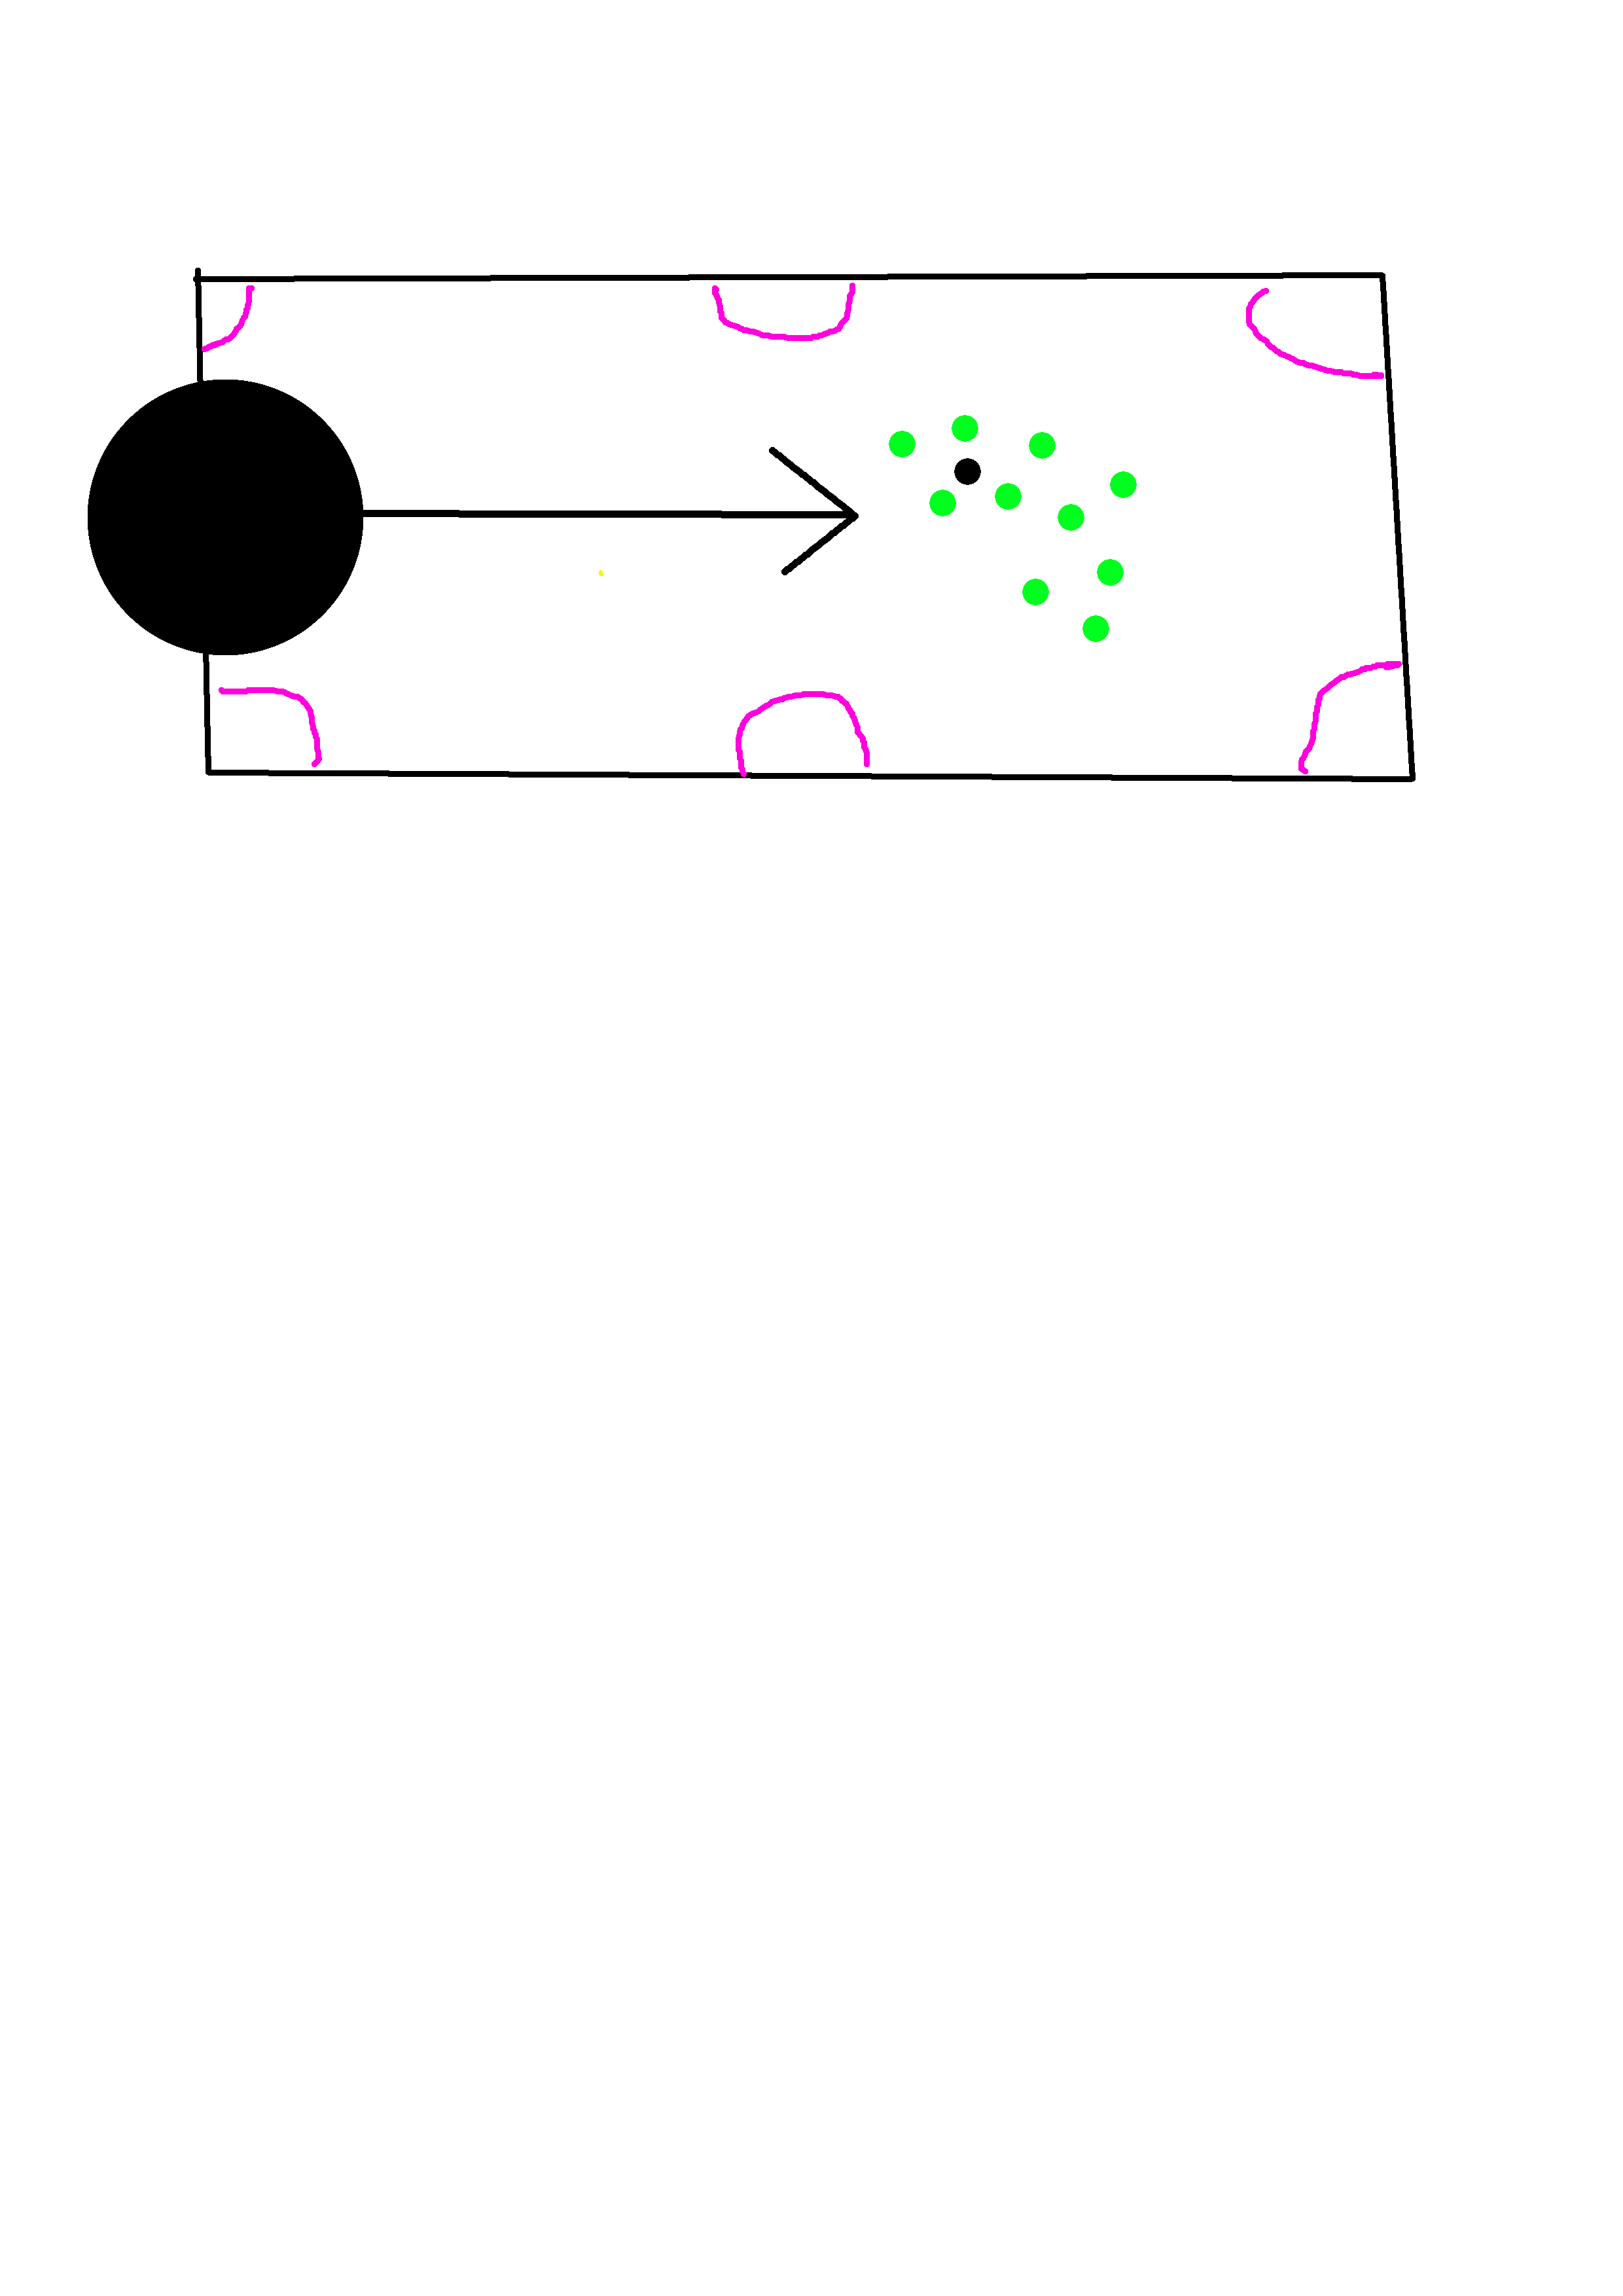
\includegraphics[trim={2cm 17cm 2cm 2cm},width=0.6\textwidth,clip]{img/game_state_4.png}
	\caption{A bowling is thrown through the middle of the field.}
	\label{fig:game_state_4}
\end{figure*}

\begin{figure*}[!htb]
	\centering
	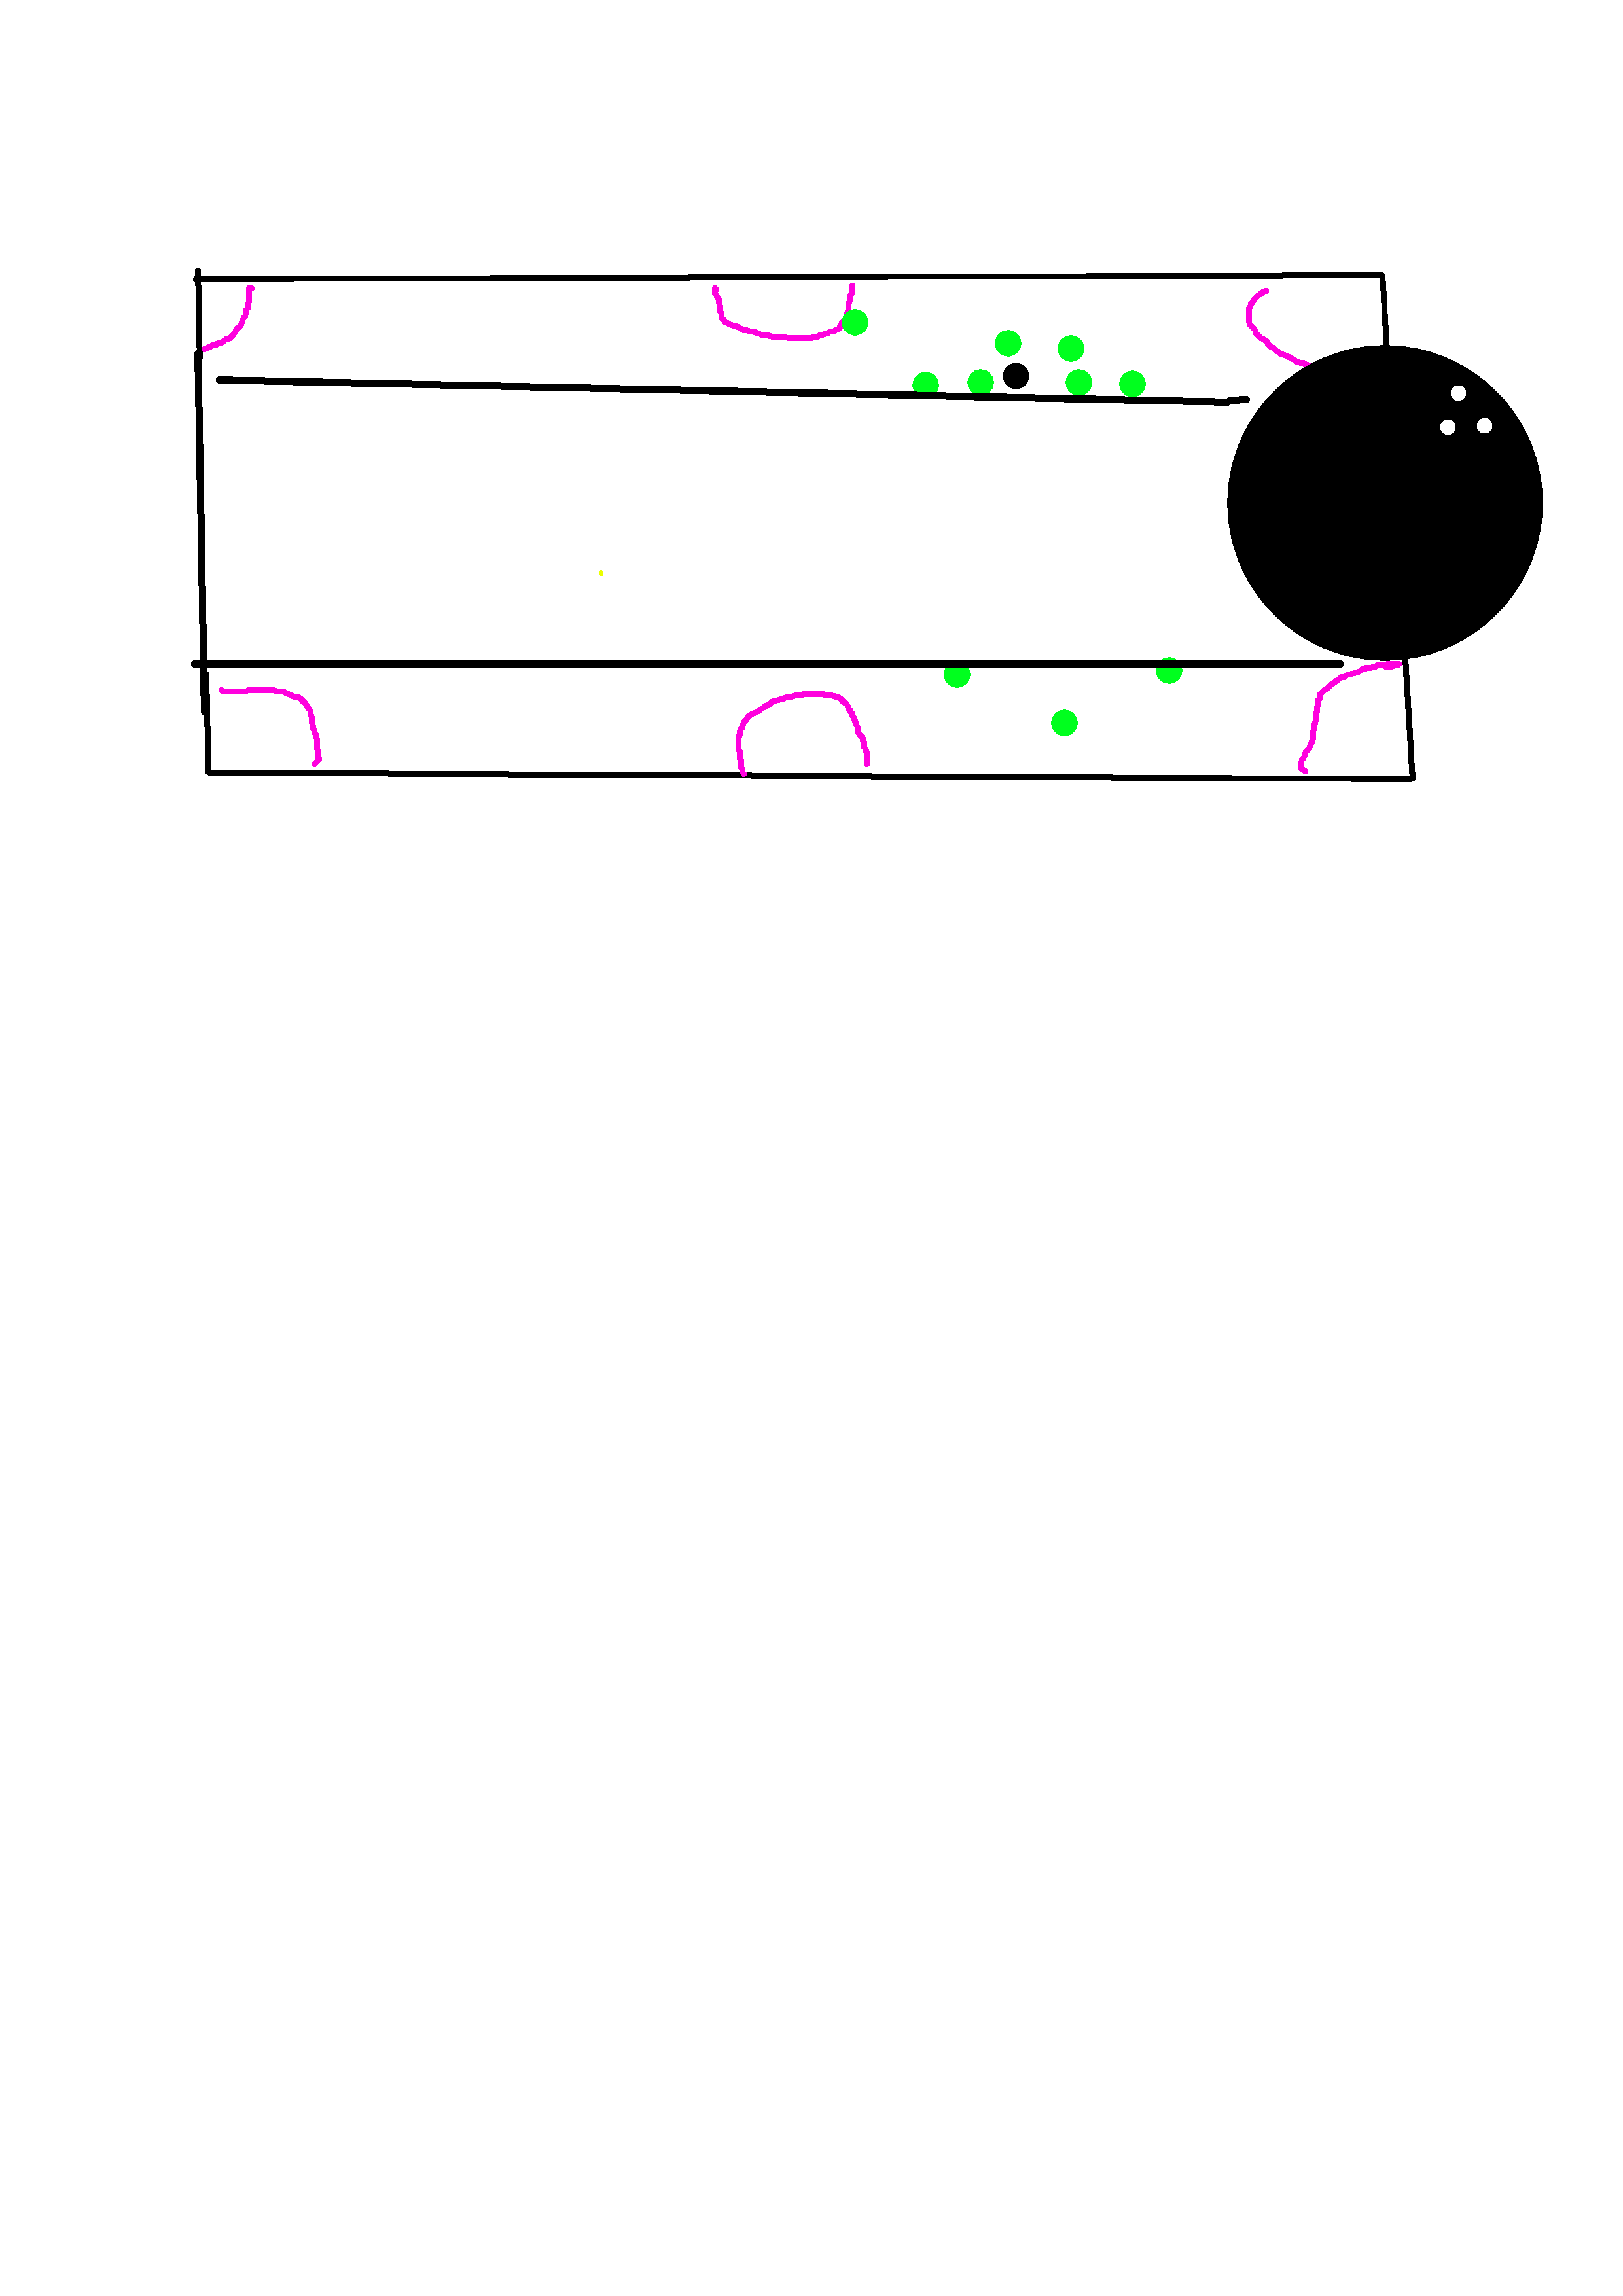
\includegraphics[trim={2cm 17cm 0cm 2cm},width=0.6\textwidth,clip]{img/game_state_5.png}
	\caption{The balls eventually settle in their new spots outside of the bowling balls impact row.}
	\label{fig:game_state_5}
\end{figure*}

 \FloatBarrier


\section{Platform}

As a platform we will primarily aim at linux as it's the easiest to develop on.\\
The main library we want to use for display/input capture is \url{https://liballeg.org} which in itself its not a game engine but just a unified back/frontend for 2D games. (Known for usage in the game factorio).



\section{List of techniques}


\subsection{Physically-based Particle Dynamics 1b}
We aim to make gravity between objects a central part of the game. It should enable the players to hit 'curved' shots through the gravitational pull of another object etc. 

\subsection{Rigid Body Dynamics 1d}
 
No game of pool would work without rigid body dynamics and their collision resolution.

\subsection{Hierarchical Transformations 4}

One of the effects we want to implement does exactly this. "Marrying" multiple balls/objects together so they move in some special relation to each other.


\subsection{Voronoi Fracture 2}

The objects that can be placed into the game field can also be glass/ice which breaks with a voronoi fracture. The effect is planned to be only visual but we may come around implementing collision with the resulting fractures as well in which case it might have gameplay effects.

\subsection{ Mass-Spring-Systems 1c}

We want to implement some spring-like behaviour but since the scale is small we don't think it qualifies as a 'mass' spring system. 


\bibliographystyle{plain}
\bibliography{references}
\end{document}

